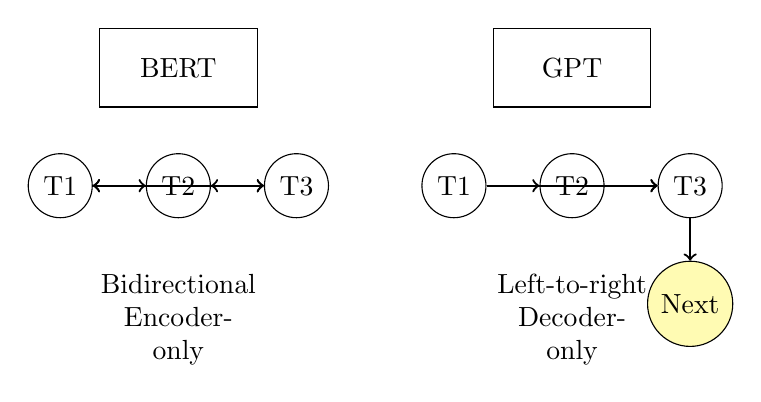
\begin{tikzpicture}[node distance=3cm, auto]
  % BERT side (left)
  \node[draw, rectangle, minimum width=2cm, minimum height=1cm] (bert_label) at (0, 4) {BERT};
  \node[draw, circle, minimum size=0.6cm] (bert_t1) at (-1.5, 2.5) {T1};
  \node[draw, circle, minimum size=0.6cm] (bert_t2) at (0, 2.5) {T2};
  \node[draw, circle, minimum size=0.6cm] (bert_t3) at (1.5, 2.5) {T3};
  
  % Bidirectional arrows for BERT
  \draw[<->, thick] (bert_t1) -- (bert_t2);
  \draw[<->, thick] (bert_t2) -- (bert_t3);
  \draw[<->, thick] (bert_t1) -- (bert_t3);
  
  \node[text width=2cm, align=center] (bert_desc) at (0, 0.8) {Bidirectional\\Encoder-only};
  
  % GPT side (right)
  \node[draw, rectangle, minimum width=2cm, minimum height=1cm] (gpt_label) at (5, 4) {GPT};
  \node[draw, circle, minimum size=0.6cm] (gpt_t1) at (3.5, 2.5) {T1};
  \node[draw, circle, minimum size=0.6cm] (gpt_t2) at (5, 2.5) {T2};
  \node[draw, circle, minimum size=0.6cm] (gpt_t3) at (6.5, 2.5) {T3};
  
  % Left-to-right arrows for GPT
  \draw[->, thick] (gpt_t1) -- (gpt_t2);
  \draw[->, thick] (gpt_t2) -- (gpt_t3);
  \draw[->, thick] (gpt_t1) -- (gpt_t3);
  
  \node[draw, circle, minimum size=0.6cm, fill=yellow!30] (gpt_out) at (6.5, 1) {Next};
  \draw[->, thick] (gpt_t3) -- (gpt_out);
  
  \node[text width=2cm, align=center] (gpt_desc) at (5, 0.8) {Left-to-right\\Decoder-only};
\end{tikzpicture}